\documentclass[12pt, final, twoside]{fithesis2}
\usepackage[inner=38mm, outer=27mm, top=37mm, bottom=48mm]{geometry}
\usepackage[utf8]{inputenc}

% searchable and copyable pdf (special characters, accents)
\usepackage{cmap}

% colours and graphics
\usepackage[usenames,dvipsnames,svgnames]{xcolor}

%\usepackage{fontspec}
\usepackage[normalem]{ulem}

\usepackage{subfig}
\usepackage[us,24hr]{datetime}
\newdateformat{mydate}{\THEDAY.\THEMONTH.\THEYEAR}
\newcommand{\verze}{  \scriptsize(v. \mydate\today\ \currenttime)}

% font
\usepackage{lmodern}
\usepackage{microtype}
\usepackage{indentfirst}
% \usepackage{verbatim}
% \usepackage{moreverb}
\usepackage{setspace} % spacing environment

\usepackage{enumitem}
\setitemize{itemsep=.5ex, topsep=.5ex, parsep=0pt, partopsep=0pt}

\usepackage[ruled,vlined,linesnumbered]{algorithm2e}
\SetAlgorithmName{Algorithm}{Algorithm}

\setlength{\algomargin}{0.5cm}

\usepackage{listings}
\lstset{
  basicstyle=\footnotesize\ttfamily,
  commentstyle=\color{Gray},
  showspaces=false,
  stringstyle=\color{orange},
  %frame=single,
  showstringspaces=false,
  keywordstyle=\bfseries\color{BrickRed},
  commentstyle=\itshape\color{Gray}
}


\newcommand{\argmax}{\operatornamewithlimits{arg\,max}}
\newcommand{\argmin}{\operatornamewithlimits{arg\,min}}

\usepackage[final]{hyperref}
\providecommand*{\Appendixautorefname}{Appendix}
\providecommand*{\problemautorefname}{Problem}
\providecommand*{\exampleautorefname}{Example}
\providecommand*{\lemmaautorefname}{Lemma}
\providecommand*{\definitionautorefname}{Definition}
\providecommand*{\algorithmautorefname}{Algorithm}
\providecommand*{\algocfautorefname}{Algorithm}
%\def\exampleautorefname{Example}
\def\sectionautorefname{Section}
\def\chapterautorefname{Chapter}

% theorems

\usepackage{framed}
\usepackage{wrapfig}

\usepackage{tabularx}

\usepackage{amsmath}
\usepackage{mathtools}  % (in texlive-latex3 package)
\mathtoolsset{showonlyrefs}

\usepackage[titletoc, title]{appendix}

%\usepackage[amsmath, amsthm, framed, thmmarks]{ntheorem}
\usepackage[amsmath, amsthm, framed]{ntheorem}

% \usepackage{amsthm}
\usepackage{tikz}
\tikzstyle{thmbox} = [rectangle, rounded corners=10, draw=gray!15, fill=gray!15, inner sep=8pt, inner ysep=1pt]
\newcommand\thmbox[1]{
  % \hspace{-8pt}
  \begin{tikzpicture}
  \node [inner sep=-10pt, inner ysep=-5pt] (box) {
    \begin{tikzpicture}
    \node [thmbox] (box){
      #1
    };
    \end{tikzpicture}
  };
  \end{tikzpicture}
}
\let\theoremframecommand\thmbox

\newcounter{common}

\usepackage{aliascnt}
\newaliascnt{theorem}{common}
\newaliascnt{definition}{common}
\newaliascnt{example}{common}
\newaliascnt{lemma}{common}
\newaliascnt{problem}{common}
\newaliascnt{corollary}{common}

\makeatletter
\renewcommand*{\thealgocf}{\arabic{chapter}.\arabic{algocf}}
\renewcommand*{\thetable}{\arabic{chapter}.\arabic{table}}
\renewcommand*{\thefigure}{\arabic{chapter}.\arabic{figure}}
\let\c@algocf\c@common
\let\c@table\c@common
\let\c@figure\c@common
\makeatother

\theoremstyle{definition}
\newshadedtheorem{definition}{Definition}[chapter]
\newtheorem{example}{Example}[chapter]
\newcommand\xqed[1]{%
  \leavevmode\unskip\penalty9999 \hbox{}\nobreak\hfill
  \quad\hbox{#1}}
\newcommand\eqed{\xqed{$\blacklozenge$}}

\theoremstyle{plain}
\newtheorem{problem}{Problem}[chapter]
\newshadedtheorem{theorem}{Theorem}[chapter]
\newtheorem{lemma}{Lemma}[chapter]
\newtheorem{corollary}{Corollary}[chapter]

\usepackage[justification=centering]{caption}
\usepackage{graphicx}

% cool symbols
\usepackage{amssymb}
\usepackage{MnSymbol}
\usepackage{wasysym}
% \usepackage{marvosym}

\usepackage{csquotes}

\usepackage[backend=biber, style=numeric, sortcites=true, sorting=none]{biblatex}

% zkratky pro zprehledneni
\usepackage[ligature]{semantic}
\mathlig{<-}{\leftarrow}
\mathlig{->}{\rightarrow}
\mathlig{<->}{\leftrightarrow}
\mathlig{==>}{\Rightarrow}
\mathlig{<==}{\Leftarrow}
\mathlig{<=}{\leq}
\mathlig{>=}{\geq}
\mathlig{...}{\dotso}

\pagestyle{plain}
\sloppy

% uncomment for compilation date and time in the header
%\renewcommand{\sectionmark}[1]{\markright{{\verze}\ \thesection\ #1}{}}

\setlength{\parskip}{.3ex plus .2ex minus .1ex}
\setlength{\parindent}{0pt}

\thesislang{en}
\thesistitle{Synthesis of Minimal Schedulers \\ for Markov Decision Processes}
\thesissubtitle{Bachelor Thesis}
\thesisstudent{Miroslav Klimoš}
\thesiswoman{false}
\thesisfaculty{fi}
\thesisyear{2012}
\thesisadvisor{RNDr. Tomáš Brázdil, Ph.D.}

\hypersetup{
    unicode=true,
    pdftitle={Synthesis of Minimal Schedulers for Markov Decision Processes},
    pdfauthor={Miroslav Klimoš},
    pdfkeywords={Markov decision process}{optimal scheduler}{minimal scheduler},
    colorlinks=true,        % false: boxed links; true: colored links
    linkcolor=BrickRed, 	% color of internal links
    citecolor=OliveGreen,   % color of links to bibliography
    filecolor=magenta,      % color of file links
    urlcolor=cyan           % color of external links
}

\begin{document}

% \FrontMatter
% \setlength{\parindent}{0pt}
% \ThesisTitlePage


% \begin{ThesisDeclaration}
% I declare that this thesis is my own work and has not been submitted 
% in any form for another degree or diploma at any university or 
% other institution of tertiary education. Information derived from the published
% or unpublished work of others has been acknowledged in the text 
% and a list of references is given.

% \AdvisorName
% \end{ThesisDeclaration}


% \begin{ThesisThanks}
% I would like to express my deepest gratitude to RNDr. Tomáš Brázdil Ph.D.
%   for being my advisor,
%   for suggesting a lot of related open problems and, in particular,
%   for his understanding when I failed to solve them. 
% I would also like to thank RNDr. Jan Krčál for all the discussions 
%   about various problems regarding continuous-time systems.
% Last but not least I thank my family for their support through my life
%   and my friends for such a great study environment.
% \end{ThesisThanks}


% \begin{ThesisKeyWords}
% stochastic processes,
% Markov decision processes, 
% continuous-time Markov decision processes, 
% time-bounded reachability, 
% optimal scheduler, 
% minimal scheduler
% \end{ThesisKeyWords}


% \begin{ThesisAbstract}
% Markov decision processes provide us with a mathematical framework
%   for modeling decision-making in randomized systems, 
%   where a scheduler controls the behavior of the system through the decisions.
% Continuous-time Markov decision processes introduce 
%   exponentially distributed time delays on the transitions to the model. 
% Time-bounded reachability objective asks for a scheduler maximizing 
%   the probability of reaching a set of goal states in a given time limit. 

% Methods for computing optimal and $\eps$-optimal schedulers
%   are available but they do not take into consideration 
%   the size of representation of such schedulers. 
% Indeed, the resulting schedulers can be very large and their potential usage
%   in embedded systems, for example, is questionable. 
% Hence, the thesis focuses on the size of schedulers and examines
%   the problem of finding a minimal optimal ($\eps$-optimal) scheduler
%   with respect to the time-bounded reachability. 

% We propose an algorithm computing a minimal $\eps$-optimal scheduler
%   for a given discrete-time system. 
% For continuous-time processes, we adopt the discretization technique 
%   to reduce the problem to the discrete-time case. 
% \end{ThesisAbstract}


% \MainMatter
% \setlength{\parindent}{0pt}

% \setcounter{secnumdepth}{1}
% \setcounter{tocdepth}{2}
% \begin{spacing}{1.2} \normalsize
% \tableofcontents
% \end{spacing}

%  \chapter{Introduction}


Code-breaking games (sometimes also called \emph{deductive games} or \emph{searching games})
  are games for two players in which the first,
  usually referred to as \emph{the codemaker},
    chooses a secret code from a given set, and the second,
  usually referred to as \emph{the codebreaker},
    strives to reveal the code by a series
    of experiments that give him partial information about the code.

\begin{wrapfigure}{r}{0.32\textwidth}
  \vspace{-5mm}
  \begin{center}
  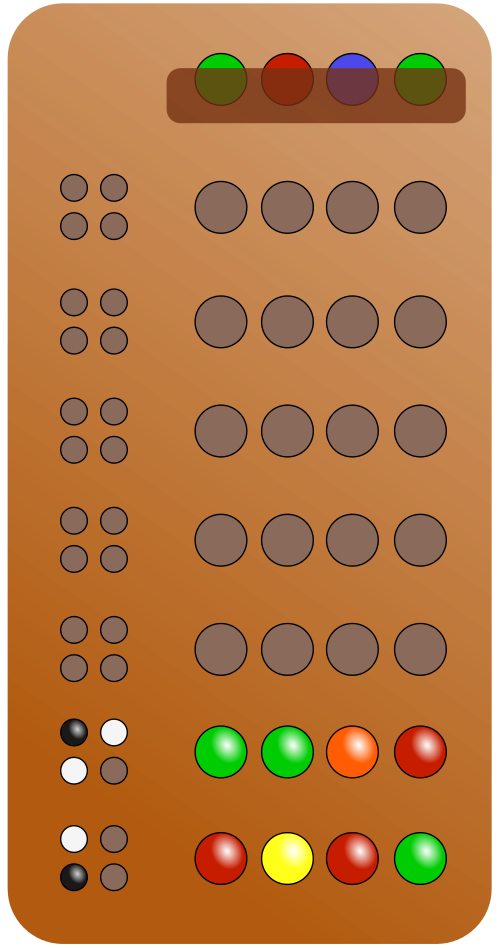
\includegraphics[width=0.25\textwidth]{pictures/mastermind.png}
  \vspace{-5mm}
  \end{center}
  \caption{Mastermind game (illustrative image)\protect\footnotemark.}
  \vspace{-5mm}
\end{wrapfigure}
\footnotetext{Image adopted from \url{http://commons.wikimedia.org/wiki/File:Mastermind\_beispiel.svg}, by Thomas Steiner under GFDL.}

The famous board game of \emph{Mastermind} is a prominent example.
The codemaker creates a puzzle for the codebreaker by choosing a
  combination of 4 coloured pegs (with colour repetitions allowed).
The codebreaker makes guesses, which are evaluated by the codemaker with
  black and white markers.
A black marker corresponds to a position at which the code and the guess matches.
A white marker means that some colour is present both in the code
  and in the guess but at different positions.

Another example is the \emph{counterfeit coin problem},
  the problem of identifying an odd-weight coin among
  authentic ones using just a balance scale.
The codemaker is not a real player here; the balance scale takes his function
  and evaluates the weighings performed by the codebreaker.
Numerous other examples can be found among various board games and logic puzzles,
 some of them being presented in the next chapter.

Code-breaking games bring many interesting problems to study.
Most importantly,
 \emph{how should the codebreaker play in order to minimize the number of experiments
   needed to undoubtedly determine the code?}
 \emph{Is there a strategy that would guarantee
   revealing the code in at most $k$ steps?}
 \emph{What strategy is optimal with respect
   to the average-case number of experiments,
   given that the code is selected
   from the given set with uniform distribution?}

Synthesis of an optimal strategy is a task computationally very intensive.
In some games, the optimal strategy might have a simple
  structure and can be described easily, such as in
  the counterfeit coin problem (see section \autoref{s:coins} for details).
In general, however, the strategy may have arbitrary structure and the only way
  to discover an optimal strategy is by considering all possible experiments
  in a given state and analysing the subproblems.

Therefore, one may prefer a suboptimal strategy or heuristics
  for experiment selection,
  which is easier to compute.
This brings another kind of problems.
Given a strategy,
  how can we compute the worst-case and the average-case number
  of experiments the strategy needs to reveal the code?

Mastermind and the counterfeit coin problem have been subjected to
heavy research and most of these questions are at least partially answered.
The exact results and summarization of the research in this area is presented
  in \autoref{ch:games}.
Nevertheless, few have been written about code-breaking games in general.
Some authors suggested general methods (and applied them on one of the games,
  e.g. \cite{cbg-stgopt, cbg-gen}),
  some vaguely stated that their approach can be applied
  to other games of the same kind but,
  to the best of our knowledge, no one has tried to
  create a general framework and provide
   results for code-breaking games in general.

Here comes this work to fill the gap.
We develop a general formalism that uses propositional logic to
  represent the secret code and the partial knowledge.
In short, the secret code is encoded as a valuation of
  a set of propositional variables
  and the codebreaker's goal is to discover the valuation
  using a series of experiments.
Each experiment can result in several outcomes,
  which are given in the form of a prepositional formula.

We study strategies for the games in general, with a focus on
  a special class of \emph{one-step look-ahead} strategies,
  strategy analysis and synthesis of an optimal strategy.
For these problems to be computationally feasible, one need to exploit
  symmetries of the game and neglect symmetric experiments during the analysis
  or strategy synthesis.
Algorithms for symmetry breaking in Mastermind
  based on graph isomorphism has been suggested in \cite{cbg-nauty}.
We generalize this approach and present
  an algorithm for elimination of symmetric experiments
  in general code-breaking games.

Main part of this thesis is a design of a computer language for
  code-breaking game specification
  and development of a computer program that
  loads a game from a file in the defined format
  and performs various tasks with the game.
We named the tool COBRA, the code-breaking game analyser.
Currently supported tasks are
\begin{itemize}
\item verify that a game specification is correct
  and sensible (overview mode),
\item simulate the game either interactively, with input from the user, or
  with decisions by specified strategies (simulation mode),
\item analyse a given strategy for experiment selection --
  compute the worst-case and average-case number of experiments needed (analysis mode),
\item synthesize the worst-case or average-case optimal strategy (optimal mode).
\end{itemize}
Using the tool, we can easily reproduce some of the known results
  for Mastermind and evaluate the same ideas in other code-breaking games.

The thesis is structured as follows.
Chapter 2 introduces several examples of code-breaking games,
  discusses known results, variants of the games and related research.
The general formalism, definitions and symmetry breaking approach
  are described in Chapter 3.
Chapter 4 is dedicated to our tool, COBRA, with description of its usage and
  abilities.
Experimental results with comparison of analysed strategies
  are presented in Chapter 5.
Finally, Chapter 6 concludes the work with many suggestions on future work
  and possible extensions of the tool.







% \input{preliminaries}
% \input{reachability}
% \input{discret}
% \input{minimal-ctmdp}
% \chapter{Conclusions}

\chapter{Code-breaking Games}

% znaceni
\newcommand{\Val}{V} % mnoz vsech valuaci
\newcommand{\val}{v} % jedna valuace
\newcommand{\numval}{\tau} % number of sat valutaions
\renewcommand{\Form}{\textrm{Form}} % mnoz vsech formuli
\newcommand{\form}{\varphi} % jedna formule
\newcommand{\aform}[1]{\form_{0..#1}} % accumulated formula

% code-breaking game
\newcommand{\game}{\mathcal{G}}
\newcommand{\Var}{X}
\newcommand{\init}{\varphi_0}
\newcommand{\Expt}{T}
\newcommand{\expt}{t}
\newcommand{\Exp}{E}
\renewcommand{\exp}{e}
%\newcommand{\Param}{\Pi}
\newcommand{\param}{p}
\newcommand{\infer}{\Phi}

% dalsi veci
\newcommand{\Perm}{\textrm{Perm}}
\newcommand{\perm}{\pi}
\newcommand{\result}{\rho}

% nep
\newcommand{\stg}{\sigma}

\newcommand{\proc}{\pi}
\newcommand{\procstg}[2]{\proc_{#1,#2}}

\newcommand{\len}{\lambda}
\newcommand{\lenstg}[2]{\len^{#1,#2}}
\newcommand{\lenmax}[1]{\len^{#1}}
\newcommand{\lenexp}[1]{\len^{#1}_\textrm{exp}}

\newcommand{\exactly}[1]{\textrm{Exactly-#1}\:}
\newcommand{\atleast}[1]{\textrm{AtLeast-#1}\:}
\newcommand{\atmost}[1]{\textrm{AtMost-#1}\:}

\section[0]{Notation}
Let $\Form_\Var$ be the set of all formulas over the set of prepositional variables $\Var$;
$\Val_\Var$ be the set of all valuations of variables $\Var$.
Formulas $\form_0, \form_1 \in \Form_\Var$ are (semantically) equivalent,
  written $\form_0 \equiv \form_1$, if
  $\val(\form_0) = \val(\form_1)$ for all $\val\in\Val_\Var$.
For a formula $\form\in\Form_\Var$, let
  $\numval_\Var(\form) = |\{ \val\in\Val_\Var \| \val(\form) = 1 \}|$
  be the number of valuations by which $\form$ is satisfied.
We often omit the index $\Var$ if it is clear from the context.

For any unary predicate $P$, $\#i\in A.P(i) = |\{ i\in A \| P(i)\}|$.
  We often omit the ``$\in A$'' part and write only $\#i.P(i)$
  if the range of $i$ is clear from the context.

Let $\Perm_\Var$ be the set of all permutations of $\Var$.

%-------------------------------------------------------------------------------
% DEF: CODE BREAKING GAME
\section{Formal definition}
\begin{definition} \label{def-game}
A \emph{code-breaking game} is a quintuple
  $\game = (\Var, \init, \Expt, \Exp, \infer)$, where
  \begin{itemize}
  \item $\Var$ is a finite set of propositional variables,
  \item $\init \in \Form_\Var$ is a satisfiable prepositional formula,
  \item $\Expt$ is a finite set of types of experiments,
  \item $\Exp \subseteq \Expt \times \Var^\star$ is an \emph{experiment} relation,
  and
  \item $\infer: \Val_\Var \times \Exp -> \Form_\Var$ is an
  \emph{inference function} such that
    \begin{enumerate}[label=(\roman*)]
    \item $\forall\val\in\Val_\Var, \exp\in\Exp$:
      $\val(\infer(\val, \exp)) = 1$ and
    \item $\forall\val\in\Val_\Var, (\expt, \param)\in\Exp, \perm\in \Perm_\Var$:
        \[
        \init \equiv \perm(\init) \;==>\;
          \infer(\val, (\expt, \perm(\param)))
          \equiv
          \perm(\infer(\val, (\expt, \param))).
        \]
    \end{enumerate}
 \end{itemize}
\end{definition}

Intuitively, the objective of the game is to find a valuation of
  variables $\Var$ by a series of experiments.
Let us call it \emph{the wanted valuation}.
The search space is reduced by formula $\init$,
  which is always known to be satisfied by the wanted valuation.

Experiments consist of a type, which is from the set $\Expt$ and a
  parametrization, which is a string of variables from $\Var$.
The experiment relation $\Exp$ specifies all permitted parametrizations
  for each type of experiment and, therefore, $\Exp$ is the set of
  all possible experiments as pairs.

The inference function is the entity that evaluates the experiment.
Given the wanted valuation and an experiment, it gives the player
  partial information about the valuation,
  in the form of a formula that is guaranteed
  to be satisfied by the wanted valuation (see condition (i)).
Put simply, condition (ii) says that if $\perm$ is a symmetry
  of the initial formula $\init$, we do not get different information
  if we permutate the variables in the parametrization of the experiment
  by $\perm$.

%-------------------------------------------------------------------------------
% EXAMPLE: FAKE-COIN PROBLEM

\begin{example}[Fake-coin problem]
Fake-coin problem with $n$ coins, one of which is fake, can be formalized as
a code breaking game
$\mathcal{F}_n = (\Var, \init, \Expt, \Exp, \infer)$, where

\begin{itemize}
\item
$\Var = \{x_1, x_2, ..., x_n, y\}$ \\
Intuitively, variable $x_i$ tells weather the coin $i$ is fake.
Variable $y$ tells weather it's lighter or heavier.

\item
$\init = \exactly{1}(\{x_1, ..., x_n\})$ \\
This is to ensure that exactly one coin is fake.

\item
$\Expt = \{\expt\}$ \\
There is only one type of experiment -- weighting the coins.

\item
$\Exp = \{ (\expt, \param) \|
  \param \in \{x_1, ..., x_n\}^{2n},
  n >= 0,
  \forall x\in\Var: \#_x(\param)<=1 \} $\\
Any sequence of variables of even length with no repetitions
  is a permitted parametrization of type $\expt$.

\item
$\infer(\val, (\expt, \param)) = \left\{
\begin{array}{ll}
(\bigvee A \wedge \neg y) \vee (\bigvee B \wedge y) &
    \textrm{if r = lighter,} \\
(\bigvee A \wedge y) \vee (\bigvee B \wedge \neg y) &
    \textrm{if r = heavier,} \\
\neg \bigvee(A\cup B) &
    \textrm{if r = equal,}
\end{array} \right.$

where
$A = \{ \param[i] \| 1 <= i <= |\param|/2 \}$,
$B = \{ \param[i] \| |\param|/2 < i <= |\param| \}$.
The conditions correspond to the result $r$ of the experiment:
\begin{itemize}
\item r = lighter if $(v(c) = 1$ for some $c\in A$ and $v(y) = 0)$
  or $(v(c) = 1$ for some $c \in B$ and $v(y) = 1)$
\item r = heavier if $(v(c) = 1$ for some $c\in A$ and $v(y) = 1)$
  or $(v(c) = 1$ for some $c \in B$ and $v(y) = 0)$
\item r = equal if $v(c) = 0$ for every $c\in A\cup B$
\end{itemize}
\end{itemize}
\end{example}

%-------------------------------------------------------------------------------
% EXAMPLE: MASTERMIND

\begin{example}[Mastermind]
Mastermind puzzle with $n$ pegs and color set $C$ can be formalized as
a code breaking game
$\mathcal{M}_{n,C} = (\Var, \init, \Expt, \Exp, \infer)$, where

\begin{itemize}
\item
$\Var = \{x_{i,c} \| 1<=i<=n, c\in C\}$. \\
Variable $x_{i,c}$ tells whether there is the color $c$ at position $i$.
For simplicity, let us use the notation $\Var_c = \{ x_{i,c} \| 1<=i<=n \}$.

\item
$\init = \bigwedge\left\{
  \exactly{1} \{x_{i,c} \| c\in C\} \| 1<=i<=n\right\}$. \\
This guarantees that there is exactly one color at each position.

\item $\Expt = \{\expt\}$.\\
There is only one type of experiment -- guessing a combination.

\item $\Exp = \{(\expt, \param) \| \param = x_{1,c_1}x_{2,c_2}...x_{n,c_n}\}$.\\
Parametrization of $\expt$ can be any string of length $n$,
$i$-th symbol of which belongs to $\{ x_{i,c} \| c \in C\}$.

\item Inference function is defined by
\begin{align*}
\infer(\val, (\expt, \param)) =\;
 & \exactly{b}\{ \param[i] \| 1<=i<=n \} \;\wedge \\
 & \exactly{t}\bigcup
      \big\{ \\
          & \{
                \atleast{k}\{ x_{i,c} \| 1<=i<=n \}
                \| 1 <= k <= \#i.(\param[i]\in\Var_c)
            \} \\
            & \| c\in C
      \big\}
\end{align*}
where $b = \# i . (\val(\param[i]) = 1)$ captures the number of black pegs
  in the response for the experiment $(t, p)$ and
  $t = \sum_{c\in C} \min( \#i.(v(x_{i,c}) = 1), \#i.(\param[i]\in\Var_c))$
  is the total number of pegs (black + white).

% TODO:
\TODO{Fakt to nejde nějak jednodušej?}
\end{itemize}
\end{example}

%-------------------------------------------------------------------------------
% DEF: STRATEGY
\section{Strategies}

\begin{definition}
A \emph{strategy} is a function $\stg: \Form_\Var -> \Exp$,
determining the next experiment for given accumulated knowledge,
such that
\[
\form_0 \equiv \form_1 ==> \stg(\form_0) = \stg(\form_1).
\]
\end{definition}

A strategy $\stg$ together with a secret valuation $\val$ induce
  a \emph{solving process}, which is an infinite sequence
\[
\procstg{\stg}{\val} = \form_0 \arrow{\exp_1} \form_1 \arrow{\exp_2}
  \form_2 \arrow{\exp_3} ...
\]
such that
$\exp_{i+1} = \stg(\form_0 \wedge \form_1 \wedge ... \wedge \form_i)$ and
$\form_{i+1} = \infer(\val, \exp_{i+1})$ for all $i\in\Nseto$.
For the sake of simplicity, let us write $\aform{k}$
instead of $\form_0 \wedge \form_1 \wedge ... \wedge \form_k$.

We define \emph{length} of the solving proces,
  denoted $|\procstg{\stg}{\val}|$
  (despite the inifinite length of the sequence),
  as the smallest $k\in\Nseto$ such that
  $\numval_\Var(\aform{k}) = 1$.
This corresponds to the situation in which we can unambigously
  determine the secret code.

Note that it always holds $\numval(\aform{k}) > 0$ because
  $\val(\aform{k}) = 1$ thanks to the condition (i)
  in Definition \ref{def-game}.

The following lemma is a straightforward consequence
  of the memory-less nature of the games. It says that once a strategy
  gives us an experiment that yields no new information, we will never more get
  any new information (using the strategy).

\begin{lemma}
If $\numval(\aform{k}) = \numval(\aform{k+1})$ for some $k\in\Nset$,
then $\numval(\aform{k}) = \numval(\aform{k+l})$ for any $l\in\Nset$.
\end{lemma}

\begin{proof}
If $\aform{k+1} = \aform{k} \wedge \form_{k+1}$
is satisfied by valuation $\val$, so must be $\aform{k}$.
Since $\numval(\aform{k}) = \numval(\aform{k+1})$, the sets of
valuations satisfying $\aform{k}$ and $\aform{k+1}$ must be exactly the same
and the formulas are thus equivalent. This implies
$\stg(\aform{k}) = \stg(\aform{k+1})$ and thus also $\form_{k+2} = \form_{k+1}$.
By induction, $\form_{k+l} = \form_{k+1}$ and $\aform{k+l} \equiv \aform{k}$
 for any $l\in\Nset$.\qed
\end{proof}

The \emph{worst-case number of experiments} $\lenmax{\stg}$
  of a strategy $\stg$ is the maximal length of the solving process
  $\procstg{\stg}{\val}$ over all valuations $\val$, i.e.
  $\lenmax{\stg} = \max_{\val\in\Val_\Var} |\procstg{\stg}{\val}|$.
We say that the strategy \emph{solves the game} if $\lenmax{\stg}$ is finite.
The game is \emph{solvable} if there exists a strategy that solves the game.

\begin{problem}
Given a code-breaking game $\game$, decide whether $\game$ is solvable.
\end{problem}

\begin{definition}
A strategy $\stg$ is \emph{optimal} if
  $\lenmax{\stg} <= \lenmax{\stg'}$ for any strategy $\stg'$.

A strategy $\stg$ is \emph{greedy} if
  for every $\form\in\Form_X$ and $\exp'\in\Exp$,
\[
\max_{\val\in\Val_\Var} \numval_\Var(\form \wedge \infer(\val, \stg(\form))) <=
\max_{\val\in\Val_\Var} \numval_\Var(\form \wedge \infer(\val, \exp')).
\]
In words, a greedy strategy minimizes
  the worst-case number of possible valuations in the next step.
\end{definition}

\begin{problem}
Given a code-breaking game $\game$,
  decide whether all greedy strategies are optimal.
This seems to be the case for Fake-coin problem (?)
  but it is not the case for Mastermind[ref].
\end{problem}

%Given a probability distribution on valuations that satisfy $\init$,
%the \emph{expected number of experiments} $\lenexp{\stg}$ of a strategy $\stg$,
%is the expected length of the solving process, i.e.
%$\lenexp{\stg} = E(\|\procstg{\stg}{\val} \|)$. (!!!)



\pagestyle{plain}
\bibliographystyle{plain}
\bibliography{biblio}

\end{document}
